\chapter{Week}
The deadline to finish the \ac{AI} demonstrator was this week Tuesday. So in the beginning of the week I worked on polishing the resnet50 example to have a smooth demo application. Furthermore, the face detection demo was also ported to the Enclustra hardware. The camera used was the same one from the Xilinx evaluation kit. A \ac{USB} 3.0 3.4 MP camera module. The reason for using the \ac{USB} camera for the demonstrator again was due to the strict timing constraints for the project. Furthermore, the camera used utilizes the standard V4L2 Linux kernel driver. This enables plug and play of the camera module and auto detection of the Petalinux \ac{OS}. Therefore, no additional driver needed to be written. The applications were written using the Xilinx \ac{SDK} against the exported root file system and libraries from the Petalinux build. In order to have access to all of the necessary functions of the \ac{DNNDK} the correct Linker flags and environmental variables needed to be set. Additionally, the utilized libraries needed to be specified. The resnet50 application and the face detection application have different requirements of course, so two applications have been implemented with the \ac{SDK}. The output of the \ac{DNNDK} compiler was included as well into the project. These output binary files are the result of the neural network compilation containing the neural network model. Compiling the whole application combines these \ac{DNNDK} binary files with the application binary file into a hybrid binary file, that can be used to run the application. Pose detection as a third demonstration application was also started to be implemented but ultimately forfeited due to the limited time. Consequently, the demonstrator has two sample applications, image classification using resnet50 and face detection, running on Enclustra hardware. All the project files and scripts necessary to replicate the design have been collected and documented for re-usability.
The second part of the week was used to prepare the data collection for the rock-paper-scissors demo. After the Synthara visit the information of how to obtain a good quality data set were shared and it was my task to create the setup for the data collection. First of all, the number of classes needed to be defined: There was one class for each of the correct symbols (rock, paper, scissors), one illegal symbol class and one background class, resulting in a total of five classes. Figure~\ref{fig:dataset_overview} summarizes the data set structure and points out the requirements for a good quality data set.
\begin{figure}[!htb]
	\centering
		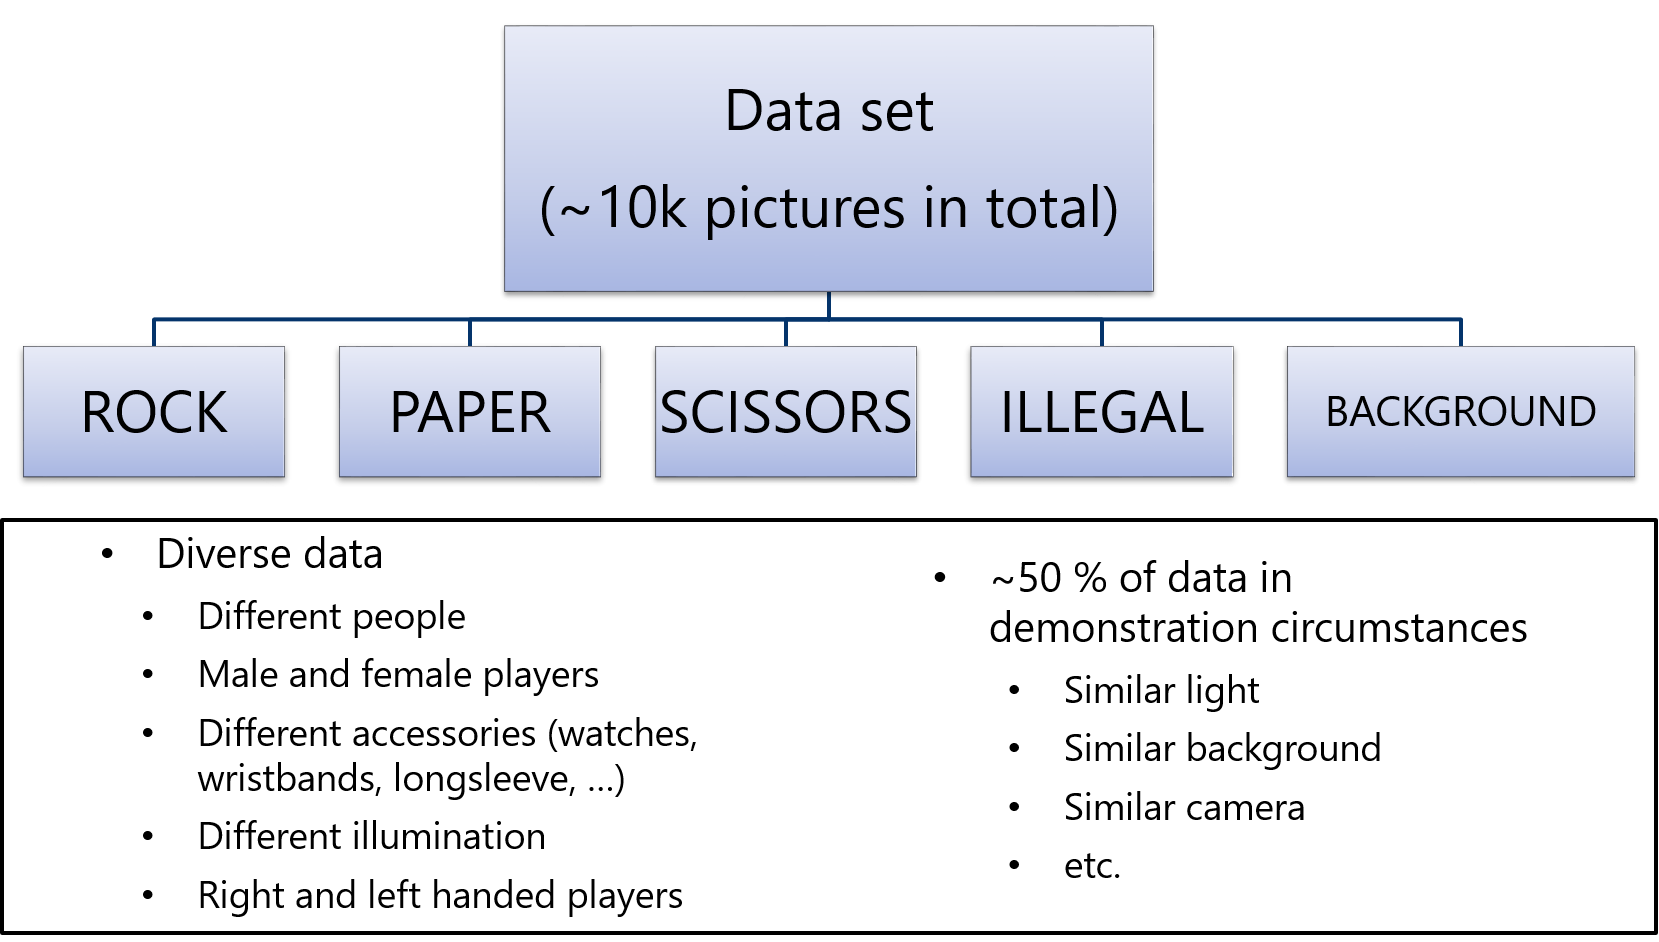
\includegraphics[width=\textwidth]{bilder/dataset_overview.png}
		\caption{Data set overview and requirements for a good quality data set}
		\label{fig:dataset_overview}
\end{figure}